%&preamble
\ifx\preambleloaded\undefined
   %&pdflatex
\documentclass[amsmath,aps,pra,amssymb,nofootinbib,notitlepage, twocolumn]{revtex4-1} % twocolumn
\bibliographystyle{apsrev}
\usepackage{dsfont} % DoubleStroke
% Pictures - ------------------------------------------------------
\usepackage{graphicx}
\usepackage{subfigure}
\usepackage[font=small]{caption}
% MATH -----------------------------------------------------------
\usepackage{amsfonts,amsmath,amssymb,mathrsfs,amsthm}
\usepackage{bm} % bolding math
\usepackage{braket} % Eg: \bra{} and \ket{} and \braket{|}
\newcommand{\norm}[1]{\left\| #1 \right\|} % Magnitude bars 
\let\conj\overline % For conjugates. 

\newcommand{\captionC}[1]{\caption{\emph{#1}}}
%\renewcommand{\thesection}{\S\arabic{section}} % starts each section with fancy section sign
\DeclareMathOperator{\Lagr}{\mathcal{L}}
\DeclareMathOperator{\Act}{\mathcal{S}}
\DeclareMathOperator{\Dif}{\mathcal{D}} % Differential over all space

\newcommand*\diff{\mathop{}\!\mathrm{d}} % Cooler integration 
\usepackage{mathtools} % For easier matrices 

% Formatting -----------------------------------------------------
\usepackage{setspace}
\usepackage{bm}

\usepackage[margin=0.4in]{geometry}
\usepackage{tikz}

\vfuzz2pt % Don't report over-full v-boxes if over-edge is small
\hfuzz2pt % Don't report over-full h-boxes if over-edge is small
\normalsize
\usepackage{color,xcolor} % Nice colours

%\SetTexturesEPSFSpecial  % use this for the Mac & Textures
%\HideDisplacementBoxes % This is for EPS files
\usepackage{cancel}


\usepackage[unicode,breaklinks]{hyperref}
\usepackage{url}
\hypersetup{
    unicode=true,
    a4paper=true,
    plainpages=false, 
    colorlinks=true,
    linkcolor=blue,
    citecolor=red,
    filecolor=black,
    urlcolor=blue
} % Colours of the links
\urlstyle{rm}
\usepackage{minted}
\usemintedstyle{pastie} %trac is default, friendly is good too
%\setstretch{1.5} % This is basically our spacing

\def\preambleloaded{}
%% end of preamble.tex

\fi
\begin{document}
\title{Characterising Conduction Properties of Indium using Helicon Waves}

\author{Eric Yeung}
\affiliation{Department of Physics, University of Toronto, Toronto M5S 1A7, Canada}
\date{\today} 

\begin{abstract} % Say something about the carrier density, and how you get it from R_H and relate it 
%The Hall coefficient and resistivity agreed well with published values.
This experiment studied the conduction properties, Hall coefficient and resistivity, of a metal with high purity. This was done by letting Helicons propagate through Indium at very low temperatures, so that phonon and electron scattering disappears, and by applying a large magnetic field to minimise the attenuation of the Helicon waves. In order to find the Hall coefficient and resistivity of Indium, the resonance frequencies and widths for the Helicons were found for fixed values of magnetic field. The Hall coefficient was found to be within 1 magnitude of Kittel's published values, although the carrier density was found to be 1 magnitude larger than Kittel's. Some of the resistivities agreed with Swenson's values, while other values agreed with White and Woods'. The Indium foil was also found to be a p-type semi-conductor because of the positive sign of the Hall coefficient. 
\end{abstract}

\maketitle

\section{Introduction}
Metals are good conductors because electrons flow freely in the metal's electron sea. So, it is impossible to have a non-zero static electric field inside a conductor. The distance that electromagnetic waves can penetrate a metal is given by the skin depth $\delta$, 

\begin{align} \label{eq:skin}
\delta = \sqrt{\frac{2\rho}{\omega \mu}}
\end{align}

where $\omega = 2\pi f_{res}$, $f_{res}$ is the frequency at which there is a resonance, and magnetic permeability $\mu = \mu_0$ since Indium is not magnetic. A Helicon is a type of electromagnetic wave that can propagate in metals with large magnetic fields. Since Helicons are low frequency electromagnetic waves, there exists resonances-- also known as modes-- of the standing waves. A phonon is the unit of energy from the vibration of atoms inside a crystal lattice.  

This experiment, introduced by Merrill et al., works because helicons propagate with higher penetration depth with the condition that the cyclotron frequency is much greater than the mean time between electron collisions \cite{c1}, which is characterised by the temperature. A lower temperature would imply a lower kinetic energy-- yielding less collisions for phonons and electrons. It was for this reason that liquid nitrogen, and even liquid helium, was used. At liquid helium temperature, T $<$ 15K, the electrons scatter off only the impurities in the metal. In this experiment, the Indium foil is 99.9999\% pure, so the electron-impurity scattering is minimised.
\vspace{2mm}

The experiment applied a large magnetic field $B$ via a superconducting magnet to produce a transverse electric field $E_y$, also known as the Hall field. The Hall coefficient is a quantity that can be studied with Helicons. The Hall coefficient $R_H$ is the ratio of the induced Hall field $E_y$ and both the current density $j_x$ and the applied magnetic field $B$. Using the equations obtained from \cite{c4},  

\begin{align} \label{eq:hallcoeff}
R_H = \frac{E_y}{j_xB} = \frac{2\mu_0}{N^2\pi B}d^2f_{res}
\end{align}

where N is the resonance, which can only be odd integers in our experiment since there is flux cancellation for even harmonics \cite{c1}, B is the static magnetic field, and d is the thickness of the Indium foil. Note that the ``current" is actually positive holes moving instead of negative electrons in the case of Indium. As $R_H > 0$ for Indium, it is a p-type semi-conductor. Indium is an intrinsic semi-conductor doped with acceptors, as opposed to being doped with donors for the case of the n-type semi-conductor.
\vspace{2mm}

Since Indium's donor is an electron acceptor, the electrons are attracted towards it-- yielding a positive region free of electrons. This positive region is known as a hole. In a p-type semi-conductor, holes are the majority carrier; electrons are the minority. The carrier density is generally defined by, 

\begin{align} \label{eq:carrierdensity}
n = \frac{1}{R_He}
\end{align}

However, in the present study, n can be thought of as the hole density. The magnetoresistance, which is the resistance of Indium that varies with the magnetic field applied, can be found from the experiment. The resistivity $\rho$ of Indium is another quantity that can be found from the experiment,

\begin{align} \label{eq:resistivity}
\rho = \frac{\mu_0}{N^2\pi}d^2 \Delta f
\end{align}

where $\Delta$f is the resonance width. Helicons can be used to study these two quantities when electrical contacts to the sample cannot be made \cite{c1}.
\vspace{2mm}

From the approach of Maxfield \cite{c6}, the angle between the Hall field and the conduction electric field is given by u, 

\begin{align} \label{eq:tangent}
u = \frac{R_H B}{\rho}
\end{align}

The Helicon wave is made up of complex and real parts. The real part, caused by $u \gg 1$, represents propagation of the wave. Conversely, the imaginary part-- in which u is not much greater than unity-- represents attenuation of the wave. The equation for the propagating Helicon wave-- for holes-- is characterised by $q_{+}$, 

\begin{align} \label{eq:holewave}
q_{+} = \sqrt{\frac{\omega \mu_0}{\rho \mu}}
\end{align}

where $\omega$ is the cyclotron frequency. The purpose of this experiment is to find the Hall coefficient and resistivity of an Indium slab by determining the resonance frequencies and resonance widths of the propagating Helicon waves. 

\section{Apparatus}
The Helicon probe, made of a drive coil and pickup coil, surrounded the Indium foil. The drive coil and pickup coil were perpendicular to each other. The drive coil was labelled by the white and red banana cables, while the pickup coil was labelled by the black and green banana cables. The circuit was arranged such that the lock-in amplifier received the signal from the pickup coil [Fig.~\ref{fig:helicon_circuit}]. 
\vspace{2mm}

The drive coil was connected to the reference generator HP 33120A ($\pm 0.05\%$), and then connected to the lock-in as well. The reference signal was used to filter out the noise from the signal of the drive coil. In order for the pickup coil signal to remain stable, it was found that the reference signal had to be $\geq 105$ mV at 100 Hz. As the frequency of the reference signal increases, so must the amplitude in order to keep the signal stable. After trial and error, 300 mV was found to be sufficient for the range of frequencies used 50 Hz -  5000 Hz. 
%\newpage
\vspace*{1mm}
\begin{figure}[H]
    \begin{center}
    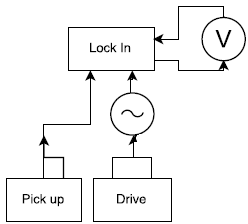
\includegraphics[scale=0.75]{helicon_circuit.png}
    \caption{Drawn block diagram of the circuit}
    \label{fig:helicon_circuit}
    \end{center}
\end{figure}
The voltmeter Wavetech BDM40 ($\pm 0.03 \%$) reads the voltage drop from the lock-in amplifier. The lab manual suggested to use an oscilloscope; however, it was not used in this experiment because the voltmeter sufficed, and an oscilloscope would introduce unwanted ground loops. The 99.9999\% pure Indium slab and its dimensions are illustrated in [Fig.~\ref{fig:indiumslab}].
%it was not used in this experiment because the voltmeter sufficed, and an oscilloscope would introduce ground loops
\begin{figure}[h!]
  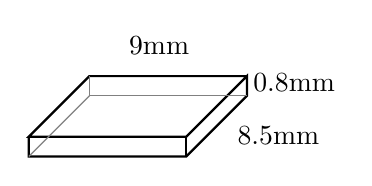
\begin{tikzpicture}
  \centering
    \draw[thick](2,0.25,0)--(0,0.25,0)--(0,0.25,2)--(2,0.25,2)--(2,0.25,0)--(2,0,0)--(2,0,2)--(0,0,2)--(0,0.25,2);
    \draw[thick](2,0.25,2)--(2,0,2);
    \draw[gray](2,0,0)--(0,0,0)--(0,0.25,0);
    \draw[gray](0,0,0)--(0,0,2);
    \draw[thick](0.5, 0.25, -1) node{9mm}; % Length
    \draw[thick](2.4, -0.5, 0) node{8.5mm}; % Width
    \draw[thick](2.6, 0.17, 0) node{0.8mm}; % Height
  \end{tikzpicture}
  \caption{The diagram of the slab was found in MP 226.}
  \label{fig:indiumslab}
\end{figure}

%\vspace*{-9mm}
With the resistance of the superconducting magnet known $R_{mag} = (9.985 \times 10^{-4}\pm 1.997 \times 10^{-7})$ $\Omega$, the voltage was read across the magnet using a digital multimeter Meterman X38R ($\pm 0.1\%$). Note that since superconductors do not have resistance, $R_{mag}$ arises from something in series with the superconductor. Ohm's law was then used to get the current. This gives a more precise reading of the current instead of reading the current off the power supply. Because the magnetoresistor in the Helicon probe was broken, the graph and fit from \cite{c1} were used to infer the magnetic field, 

\begin{align} \label{eq:magfit}
B = \left(324 \pm 2 \hspace{2mm} G\cdot A^{-1} \right) \cdot I
\end{align}

The resistances of the drive and pickup coils were recorded at room temperature, after they were dipped in liquid nitrogen, and after they were dipped in liquid helium [Table.~\ref{table:1}].   

\begin{table}[H]
\caption{Resistances of the Drive and Pickup Coils at different Temperatures}
\centering
\begin{tabular}{l l l}
\hline % Perfect spacing Eric! Thanks Eric!
\hline
Temperature (K) & $R_{drive} (\Omega)$ & $R_{pick up} (\Omega)$ \\ \hline
\hspace{8mm} 293 & \hspace{2mm} 99.54 & \hspace{2mm} 173.31  \\ 
\hspace{8.5mm} 77 & \hspace{2mm} 13.87 & \hspace{2.5mm} 23.20 \\ 
\hspace{8mm} 4.2 & \hspace{2.5mm} 1.69 & \hspace{3mm} 2.43 \\ 
\hline \hline
\end{tabular}
\label{table:1}
\end{table}

%\vspace{-5mm}
These values confirmed that the drive and pickup coils were indeed connected and continuous. Then, the two sets of measurements were made. The frequency from the reference signal was first fixed, and the magnetic field was varied. Then, to find higher order resonances, the magnetic field was fixed, and the frequency was allowed to vary. The voltage amplitude from the pickup coil was recorded and graphed for each case-- the peaks and peak widths in the graphs lead to the calculation of both the Hall coefficient and the resistivity. 
%\vspace{-5mm}
\newpage
\section{Results}
To get an idea for which frequencies to look for, a preliminary run was done with fixed frequency and varying magnetic field. It was found that almost each frequency had a resonance, depicted by a peak, except for 400 Hz, shown in [Fig.~\ref{fig:fixed_frequencys}].

\begin{figure}[H]
    \begin{center}
    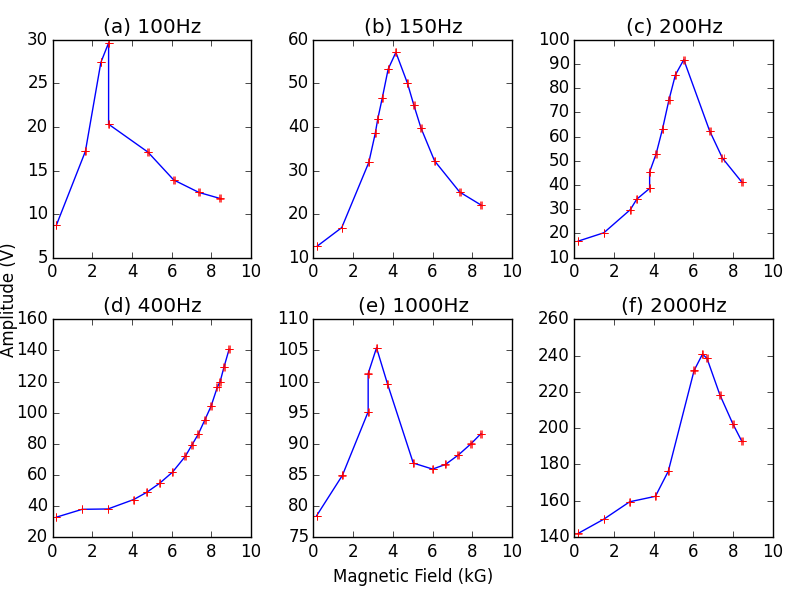
\includegraphics[scale=0.46]{fixed_frequency.png} % 0.45 scale might work for 2 column
    \caption{Varying the magnetic field while fixing frequency. (d) behaves strangely as there is no peak, only exponential growth. This can be explained by the peak being at a higher value of magnetic field, or the fact that there is no resonance at 400 Hz.}
    \label{fig:fixed_frequencys}
    \end{center}
\end{figure}

The two resonances, shown in the fixed magnetic field graphs, have half-wavelengths of 1 and 3. For B = 3244.87 G, the N = 1 and N = 3 resonances were found to be at $f_{res} = 136$ Hz and $f_{res} = 1100$ Hz respectively. The resonance widths were also found to be $\Delta$f = 60Hz for N = 1, but the N = 3 resonance was not well defined so the resonance width was not clear. See [Fig.~\ref{fig:freq_10A}].

\begin{figure}[H]
    \begin{center}
    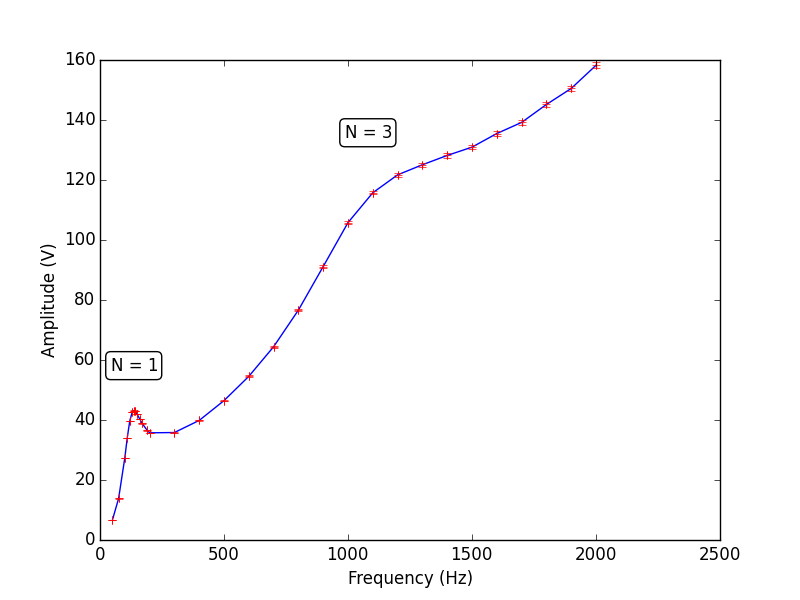
\includegraphics[scale=0.46]{freq_10A_notitle.png}
    \caption{Varying frequency for B = 3244.87 G}
    \label{fig:freq_10A}
    \end{center}
\end{figure}

Similarly for B = 5191.79 G shown in [Fig.~\ref{fig:freq_16A}], the N = 1 and N = 3 resonances were found to be at $f_{res} = 203$ Hz and $f_{res} = 1800$ Hz respectively. The resonance widths were $\Delta$f = 80Hz and $\Delta$f = 200 Hz respectively.

\begin{figure}[H]
    \begin{center}
    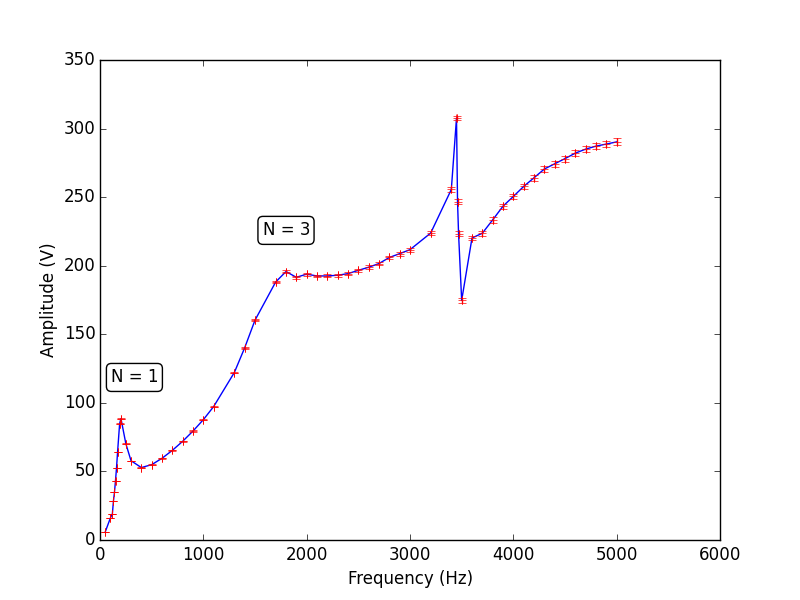
\includegraphics[scale=0.46]{freq_16A_notitle.png}
    \caption{ Varying frequency for B = 5191.79 G. Note that there is a spike around 3450 Hz. This might represent a higher order resonance (N = 5, \ldots) or just an outlier.}
    \label{fig:freq_16A}
    \end{center}
\end{figure}

\vspace*{-6mm}
Lastly for the B = 8436.65 G scenario shown in [Fig.~\ref{fig:freq_26A}], the N = 1 and N = 3 resonances were found to be at $f_{res} = 321$ Hz and $f_{res} = 2730$ Hz respectively. The resonance widths were also found to be $\Delta$f = 30 Hz and $\Delta$f = 600 Hz respectively for the N = 1 and N = 3 resonances. The graphs and data suggest that the resonance frequencies and widths are proportional to the magnetic field. 

\begin{figure}[H]
    \begin{center}
    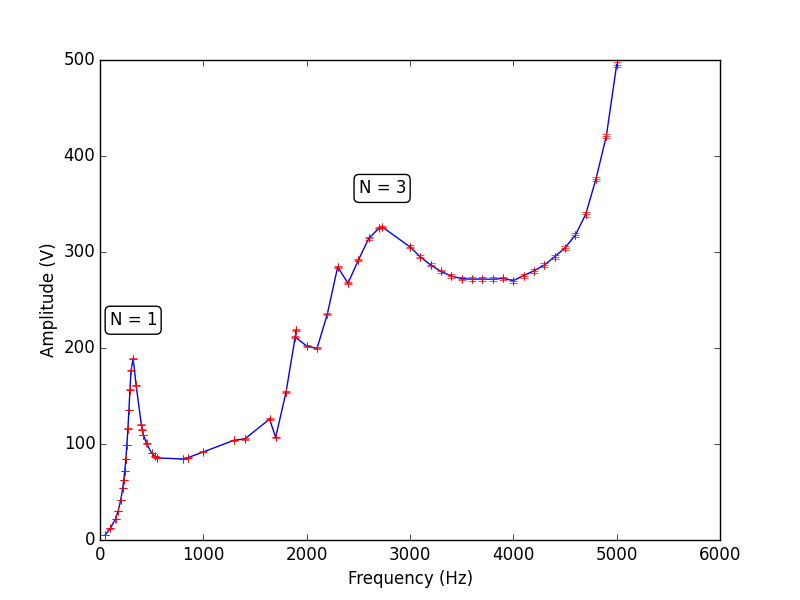
\includegraphics[scale=0.46]{freq_26A_notitle.png}
    \caption{Varying frequency for B = 8436.65 G}
    \label{fig:freq_26A}
    \end{center}
\end{figure}

\vspace*{-10mm}
Note that there are some spikes leading to the N = 3 resonance in the B = 8436.65 G case, but this cannot be another resonance (i.e., N = 2) since there is flux cancellation for even resonances \cite{c1}. There are higher order resonances, but the N = 1 resonances are the most well-defined. So the plots were truncated at 1000 Hz to show only the first resonances for each magnetic field [Fig.~\ref{fig:N1_resonance_plot}]. 

\begin{figure}[H]
    \begin{center}
    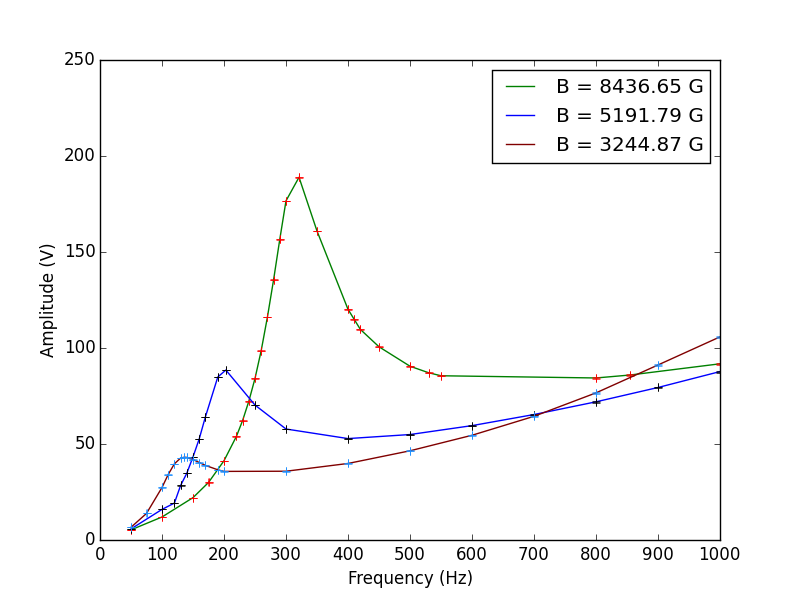
\includegraphics[scale=0.46]{N1_resonance_plot_notitle.png}
    \caption{Truncated Plot for the N = 1 resonances}
    \label{fig:N1_resonance_plot}
    \end{center}
\end{figure}

The Hall coefficients $R_H$ were calculated from [Eq.~\ref{eq:hallcoeff}], and the resistivities $\rho$ were calculated from [Eq.~\ref{eq:resistivity}]. The resisitivities were calculated for only the N = 1 resonances, since all of the N = 1 resonance widths $\Delta$f were well defined. And for consistency, the Hall coefficients were calculated for only the N = 1 resonances as well. The hole densities were computed using [Eq.~\ref{eq:carrierdensity}]. And the results, for the N = 1 resonance, were recorded in [Table.~\ref{table:2}].
\vspace{4mm}
\begin{table}[H]
\caption{Results for Hall coefficient, resistivity and carrier density for different magnetic fields.}
\centering
\begin{tabular}{l l l l}
\hline % Wow! Such good spacing again!
\hline
B (G) & $R_H \hspace{1mm}(\pm 3\% \hspace{1mm} \frac{\text{m}^3}{\text{C}})$ & $\rho \hspace{1mm} (\pm 3\% \hspace{1mm} \Omega \cdot$m) & Hole Density ($\pm 3\%$)\\ \hline
3245 & $5.64 \times 10^{-10}$ & $7.78 \times 10^{-12}$ & \hspace{5mm} $1.11 \times 10^{28}$ \\ 
5192 & $8.42 \times 10^{-10}$ & $2.07 \times 10^{-11}$ & \hspace{5mm} $7.41 \times 10^{27}$ \\ 
8436 & $1.33 \times 10^{-9}$ & $1.56 \times 10^{-11}$ & \hspace{5mm} $4.70 \times 10^{27}$ \\ \hline
\text{Average} & $9.12 \times 10^{-10}$ & $1.48 \times 10^{-11}$ & \hspace{5mm} $7.74 \times 10^{27}$ \\
\hline \hline
\end{tabular}
\label{table:2}
\end{table}

A quantity that Merrill et al. suggested to calculate was the quality constant Q $= f_{res}/\Delta f$. This value is dimensionless and resembles a slope. It can also be thought as the sharpness of the specific resonance peak. The sharper the peak, the more well defined the resonance is. For 3244 G, 5192 G, and 8436 G, the quality constant was 4.53, 2.54, and 5.35 respectively. % Polish this up

%\clearpage
%\newpage
\section{Discussion}

This experiment followed closely Merrill et al.'s; although unlike Merrill et al., data for the Helicon resonances as a function of temperature was not taken. This is because there was no reliable way to measure the temperature near 4.2 K if the Helicon probe was pulled out of the helium dewar. Compared to copper which has a resistivity $1.68 \times 10^{-8}$ $\Omega \cdot$m at 293 K, Indium has a resistivity $8.37 \times 10^{-8}$ $\Omega \cdot$m at 293 K which is typical of metals. The resistivity can be explained by the shape of the Fermi surface of Indium, but this is beyond the scope of the experiment.  

With the resistivity of indium at 293 K known to be $8.37 \times 10^{-8}$ $\Omega \cdot$m, it is reasonable to say that the resistivity at 273 K is of order $\mathcal{O}(10^{-8})$. From Table 2 in Swenson \cite{c5}, R/$R_{273.2}$ = 0.001 at 4.2 K. So the resistivity at 4.2 K is $\mathcal{O}(10^{-3}) \cdot \mathcal{O}(10^{-8}) = \mathcal{O}(10^{-11})$ according to Swenson.  
 
Similarly in White and Woods' experiment \cite{c2}, they found that $R_{4.2}/R_{273} \sim 10^{-4}$. So the resistivity at 4.2 K is $\mathcal{O}(10^{-4}) \cdot \mathcal{O}(10^{-8}) = \mathcal{O}(10^{-12})$ according to White and Woods. In contrast, White and Woods' value is 1 order of magnitude smaller than Swenson's. The resistivities associated with the higher magnetic fields B = 8436 G and B = 5192 G are of the order $\mathcal{O}(10^{-11})$ which is within 1 magnitude of Swenson's values. The lowest magnetic field B = 3244 G is of the order $\mathcal{O}(10^{-12})$ which is within 1 magnitude of White and Woods' values. As expected from a metal, the resistivity of the Indium sample is lower at 4.2 K than 293 K. 

As all my values of $R_H$ were positive, Indium can be classified as a p-type semi-conductor with electron holes as carriers. This is because $R_H > 0$ implies a positive charge on the carriers, which in this case are just holes. Kittel's published value for the Hall coefficient of Indium is $R_H = +1.602 \times 10^{-10}$ $\text{m}^3/\text{C}$ \cite{c3}, the closest empirical value in this experiment was at B = 3245 G which is $R_H = (+5.64 \times 10^{-10} \pm 1.128 \times 10^{-11})$ $\text{m}^3/\text{C}$. This is unexpected as one would expect higher magnetic fields giving better results, since a larger magnetic field would imply a larger Hall angle tangent [Eq.~\ref{eq:tangent}] such that $u \gg 1$. This results in less attenuation and more propagation of the Helicon wave; thus, leading to better results. 

In theory, the Hall coefficient should be the same for every value of the magnetic field. The main experimental error was taking less data points around some of the peaks due to time constraints, resulting in smaller quality constants and less sharp, well defined resonances. Consequently, any deviation in $f_{res}$ can change the value of the Hall coefficient. Kittel's value of carrier density is $1.17 \times 10^{26}$, while mine averages to around $7.74 \times 10^{27}$ which is 1 magnitude higher. Since the carrier density is calculated from the Hall coefficient, any deviation in $R_H$ can change the value of the carrier density as well.    

\section{Conclusion}

After letting Helicons propagate through Indium and measuring the resonance frequencies and widths, the average Hall coefficient was found to be $(+9.12 \times 10^{-10} \pm 2.74 \times 10^{-11})$ $\text{m}^3/\text{C}$, which is within 1 magnitude of Kittel's. The average resistivity was found to be $(1.48 \times 10^{-11} \pm 4.41 \times 10^{-13})$ $\Omega \cdot$m, which agrees more with Swenson's values $\mathcal{O}(10^{-11})$ than White and Woods' $\mathcal{O}(10^{-12})$. The average hole density was found to be $7.74 \times 10^{27} \pm 2.32 \times 10^{26}$ compared to the carrier density $1.17 \times 10^{26}$ quoted in Kittel's \cite{c3}.    
The metal, Indium, was identified as a p-type semi-conductor because of the positive sigh of $R_H$. It follows that the charge carriers in Indium are positive, also known as holes. 

\clearpage
\begin{thebibliography}{1} 
\bibitem{c1}J. Pitre, ``Helicons in Metals Lab Manual" (2012), 2-13%; \href{http://www.physics.utoronto.ca/~phy326/hel/hel.pdf}{Advanced undergraduate laboratory}
\bibitem{c2}G.K. White, S.B. Woods, ``Indium Resistance Thermometer; 4 to 300K", Rev. Sci. Instr. {\bf 28}, 638, 1957. 
\bibitem{c3}C. Kittel,``Introduction to Solid State Physic'', 6th edition (1986), 150-151
\bibitem{c4}J. R. Merrill, D. Pierce, and D. Giovanielli, ``A Helicon Solid-State Plasma Experiment for the Advanced Laboratory'', Amer. J. Phys. {\bf 38} (1970), 417-421
\bibitem{c5}C.A. Swenson, ``Properties of Indium and Thallium at Low Temperatures'', Phys. Rev. {\bf 100}, 1607, 1955.  
%\bibitem{c6}N.W. Ashcroft and N.B. Mermin, ``Solid State Physics'', (1976), 14-15
\bibitem{c6}B. W. Maxfield, ``Helicon Waves in Solids", Amer. J. Phys. {\bf 37} (1969), 241-269 
\end{thebibliography}

\end{document}
